\chapter{Signal and Background processes}
\label{chap:sigbkg}

The details of the signal and the background modeling in the Monte-Carlo simulation are discussed in this chapter.

\section{Signal process}
The signal samples are generated with two on-shell V bosons (V is Z or W), one of which decays leptonically, and the other hadronically (semi-leptonic final states).
Theoretically, VBS processes shown in Fig~\ref{fig:feynmanVBS} cannot be distinguished from the other electroweak VV+jj proceses like diagrams shown in Fig~\ref{fig:feynmanEWKnonVBS2} and Fig~\ref{fig:feynmantZb}, for the gauge invariant conservation, hence they are generated altogether as electroweak (EW) VV+jj production.

%% feynman diagrams, VBS
\begin{figure}[H]
\begin{center}
 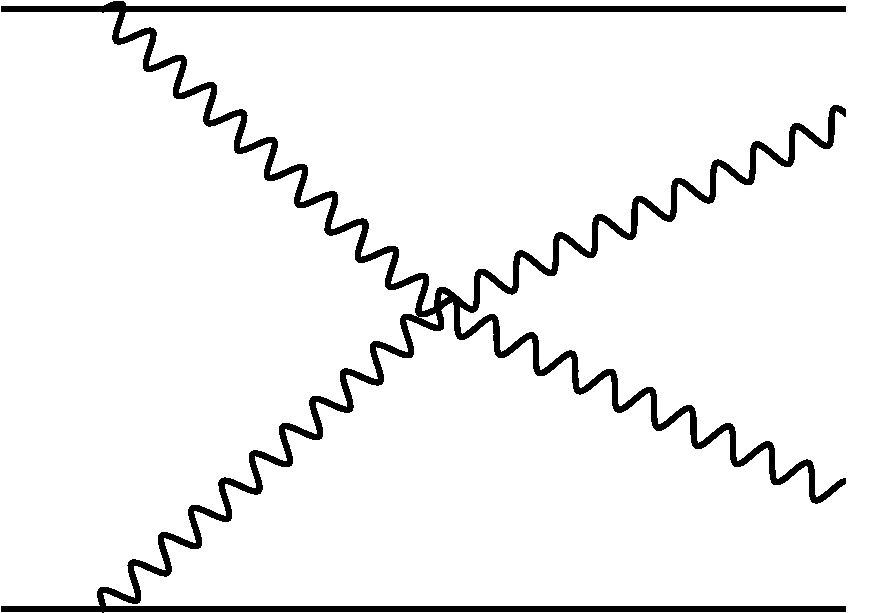
\includegraphics[width=0.3\textwidth,keepaspectratio]{figures/samples/feynVBS2.pdf}
 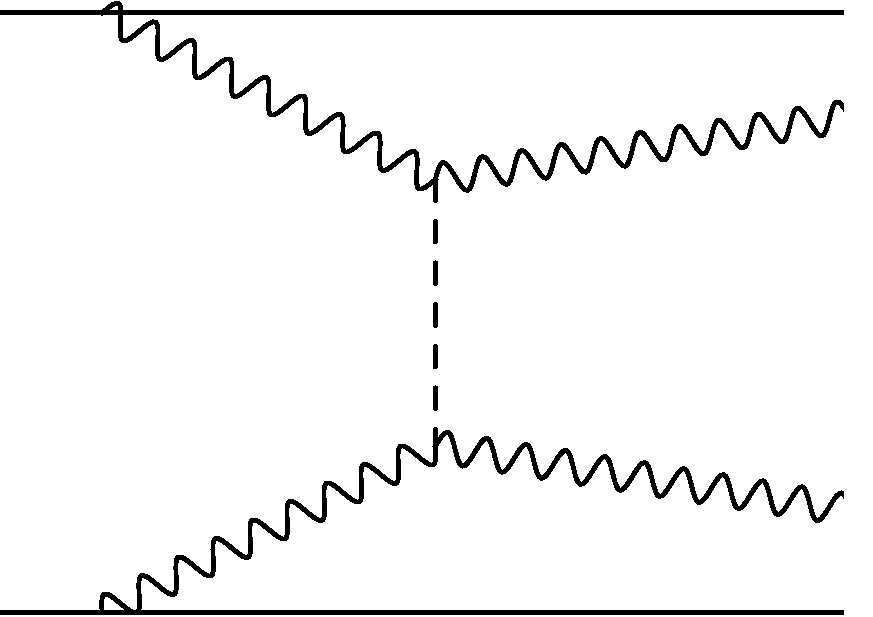
\includegraphics[width=0.3\textwidth,keepaspectratio]{figures/samples/feynVBS1.pdf}
 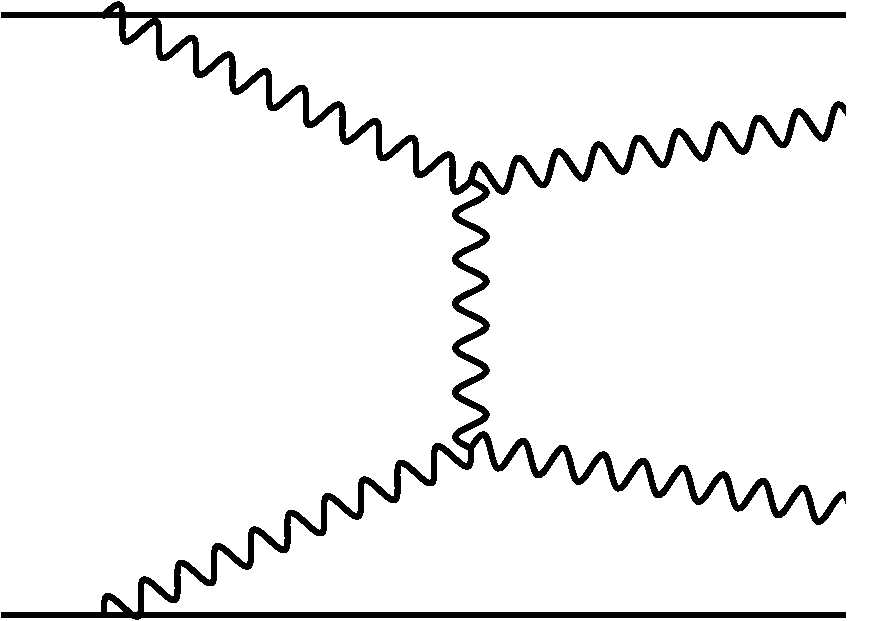
\includegraphics[width=0.3\textwidth,keepaspectratio]{figures/samples/feynVBS3.pdf}
 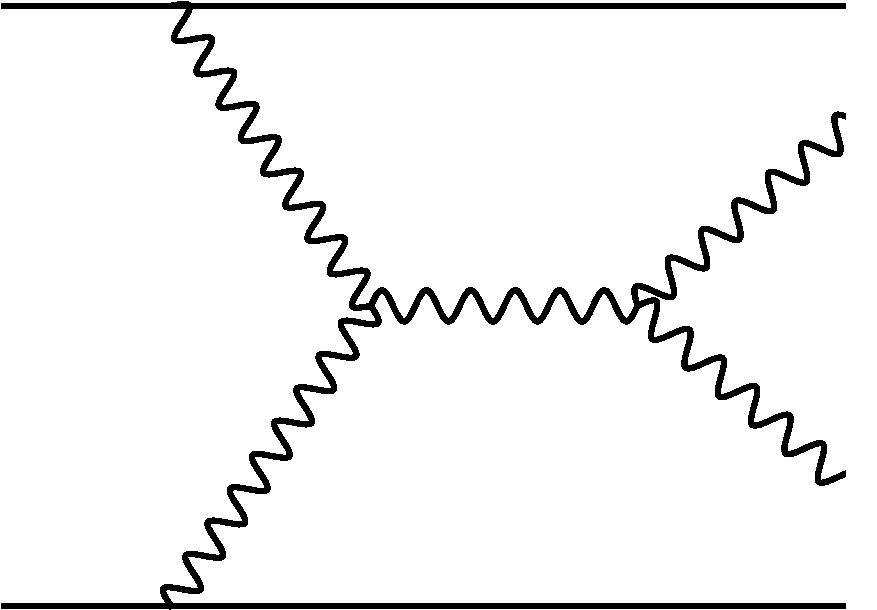
\includegraphics[width=0.3\textwidth,keepaspectratio]{figures/samples/feynVBS4.pdf}
 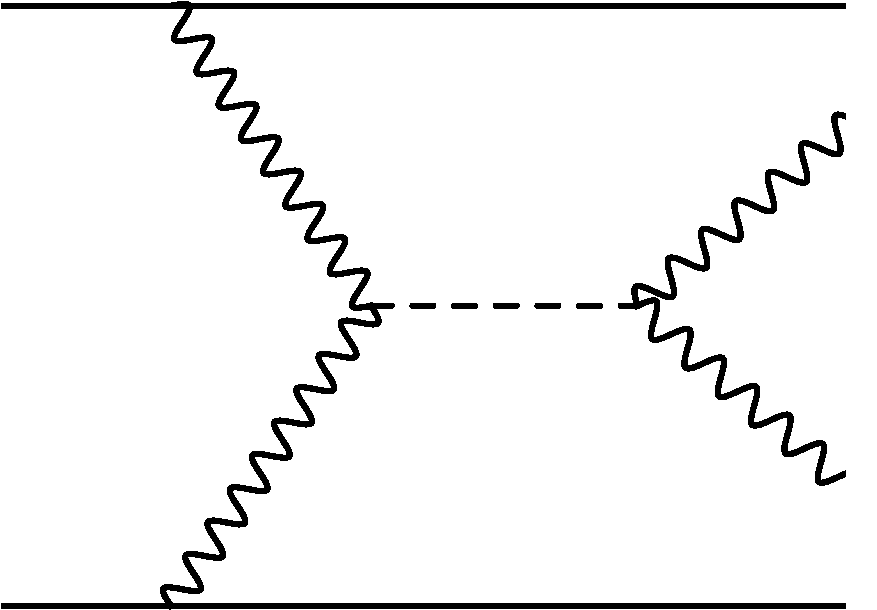
\includegraphics[width=0.3\textwidth,keepaspectratio]{figures/samples/feynVBS5.pdf}
\caption[f]{
VBS diagrams contribute to the signal.  
The dashed line represents the Higgs boson.The decay products of the bosons are not shown.
}
\label{fig:feynmanVBS}
\end{center}
\end{figure}

The non-VBS diagrams, which do not includes the boson scattering, shown in Figure~\ref{fig:feynmanEWKnonVBS1}, \ref{fig:feynmanEWKnonVBS2}. 

%% feynman diagrams, non-VBS
\begin{figure}[H]
\begin{center}
 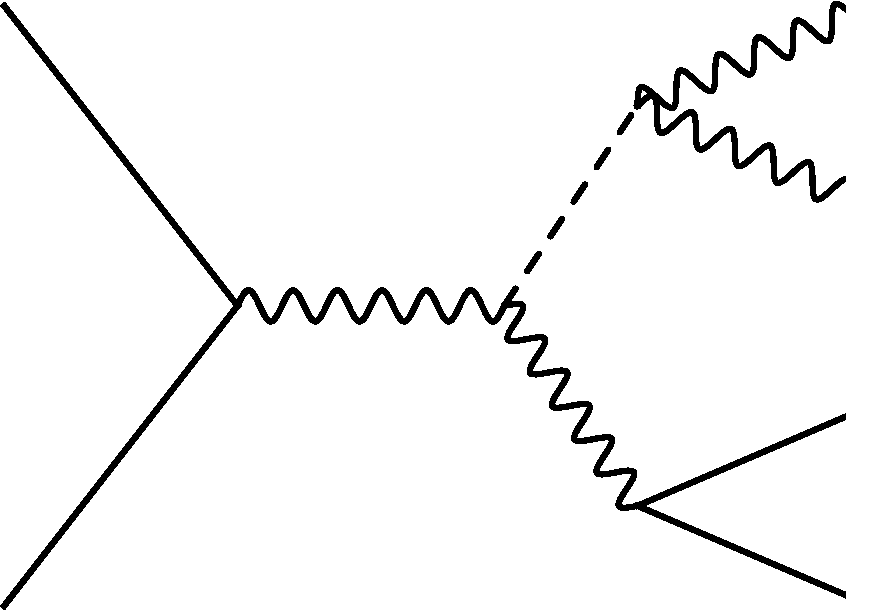
\includegraphics[width=0.30\textwidth,keepaspectratio]{figures/samples/feynEWKnonVBS3.pdf}
 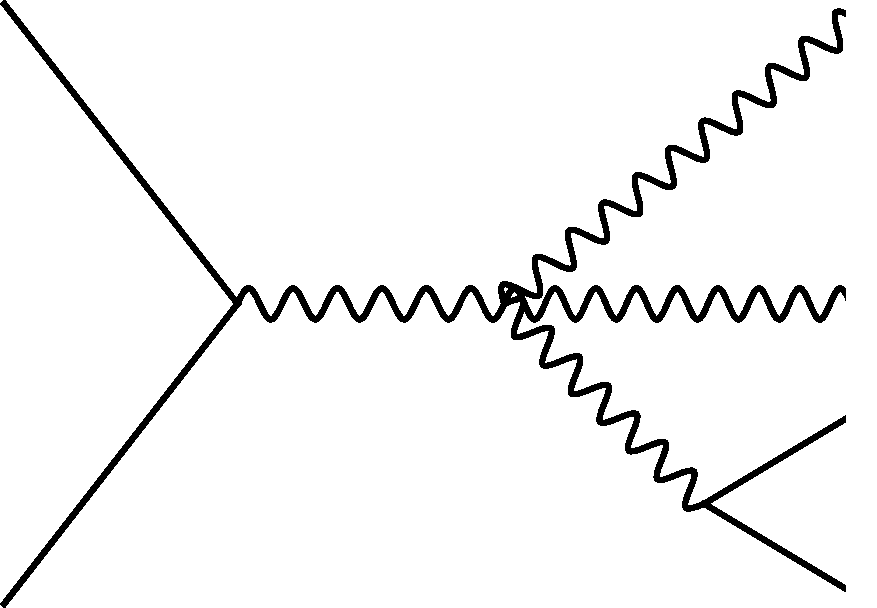
\includegraphics[width=0.30\textwidth,keepaspectratio]{figures/samples/feynEWKnonVBS4.pdf}\\
 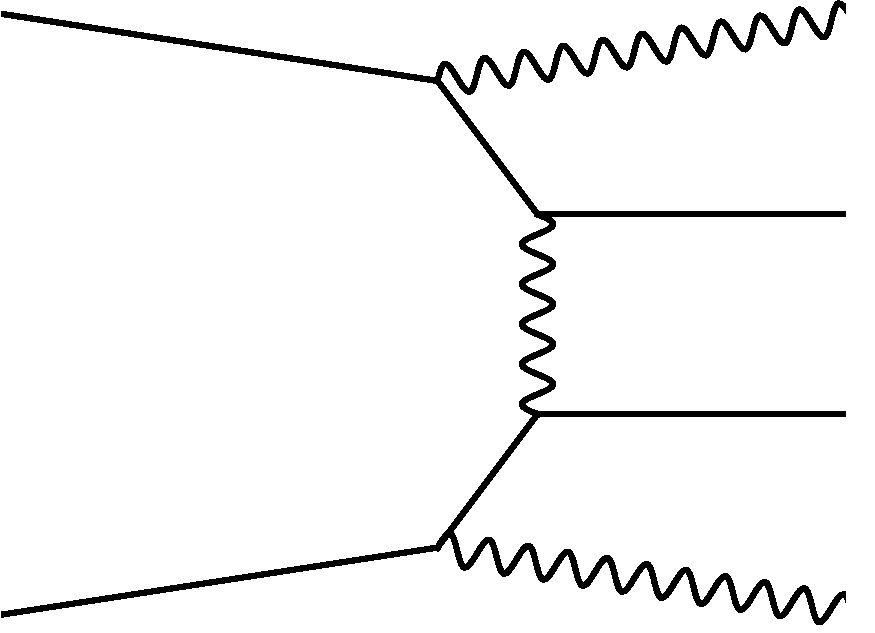
\includegraphics[width=0.30\textwidth,keepaspectratio]{figures/samples/feynEWKnonVBS5.pdf}
 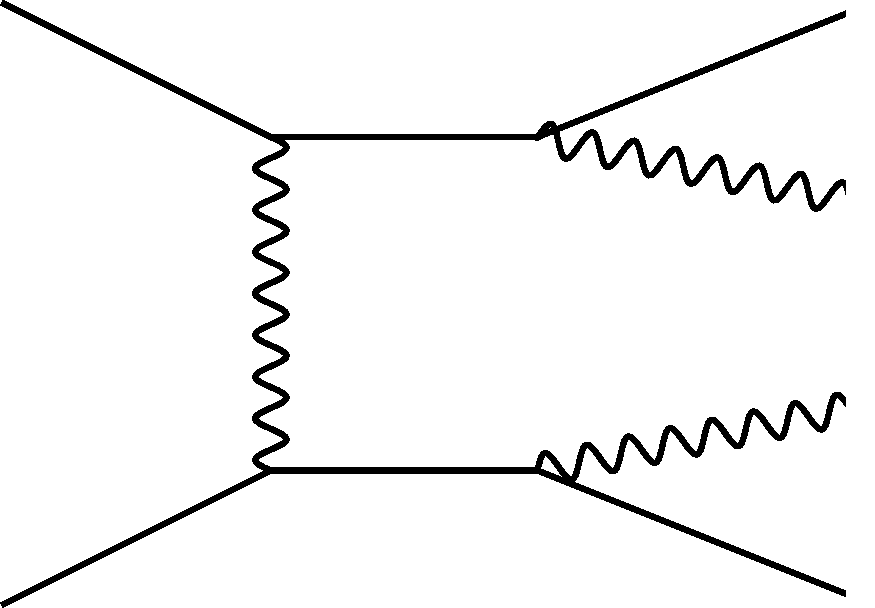
\includegraphics[width=0.30\textwidth,keepaspectratio]{figures/samples/feynEWKnonVBS6.pdf}
 \caption[f]{
non-VBS diagrams contribute to the signal. 
}
 \label{fig:feynmanEWKnonVBS1}
\end{center}
\end{figure}
\begin{figure}[H]
\begin{center}
 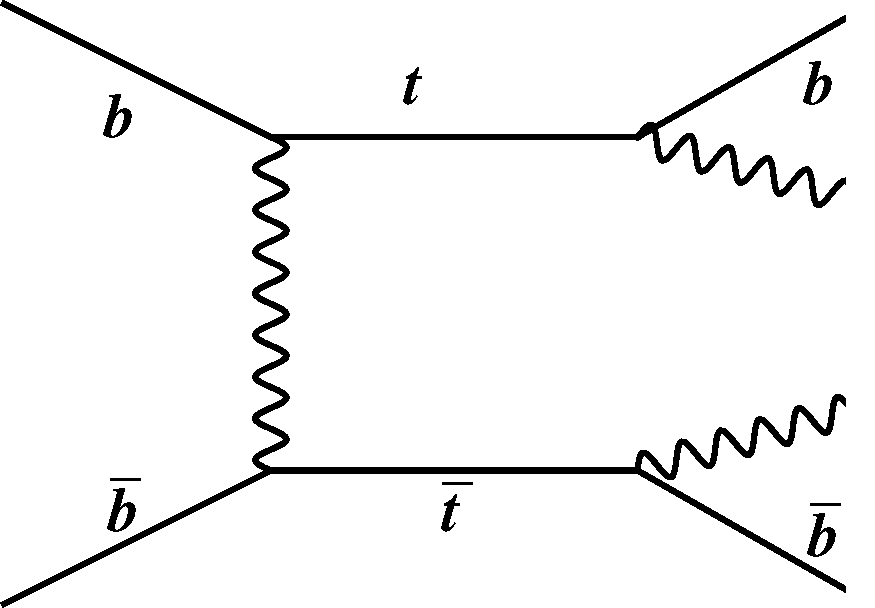
\includegraphics[width=0.3\textwidth,keepaspectratio]{figures/samples/feynEWKnonVBS1.pdf}
 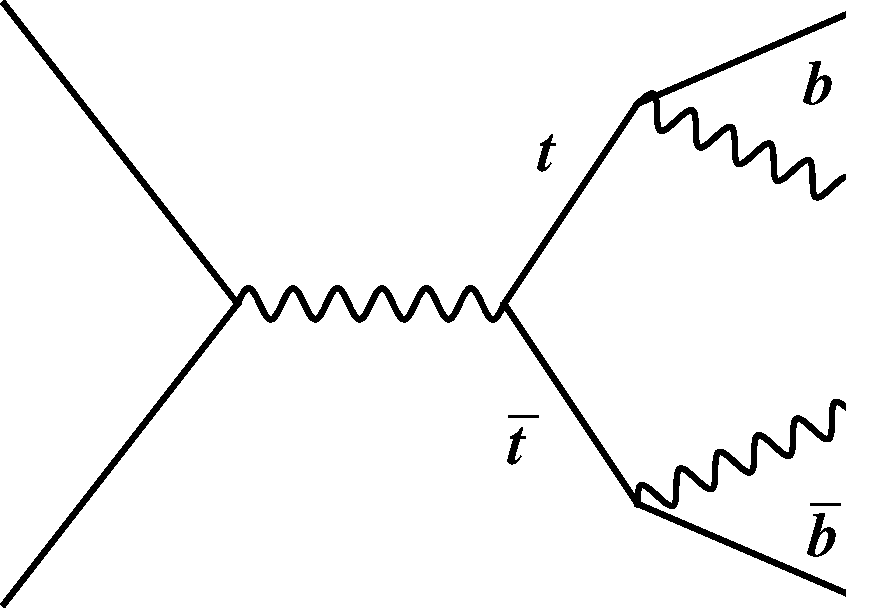
\includegraphics[width=0.3\textwidth,keepaspectratio]{figures/samples/feynEWKnonVBS2.pdf}
 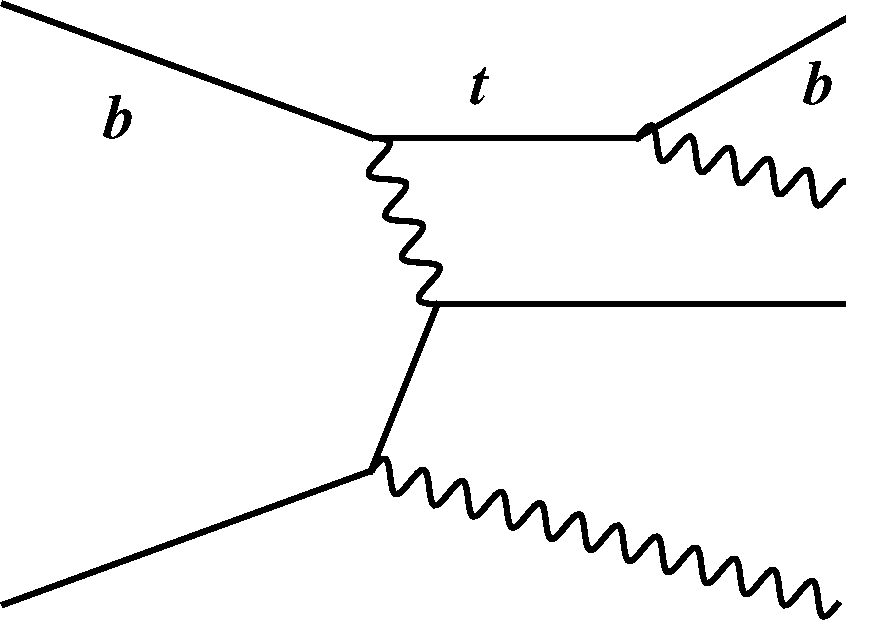
\includegraphics[width=0.3\textwidth,keepaspectratio]{figures/samples/feynEWKnonVBS7.pdf}
 \caption[f]{
non-VBS diagrams contribute to the signal, which include top.
}
\label{fig:feynmanEWKnonVBS2}
\end{center}
\end{figure}

Especially the contribution from electroweak ttbar process is included about 50~\% of the whole EW VV+jj signal samples, which can be suppressed by applying b-veto (not requiring the b-tagged jets). After applying b-veto in the event selection, there is still non-negligible contributions from tZb process, which is shown in Figure~\ref{fig:feynmanVBS}. 

%% feynman diagram, tZb
\begin{figure}[H]
\begin{center}
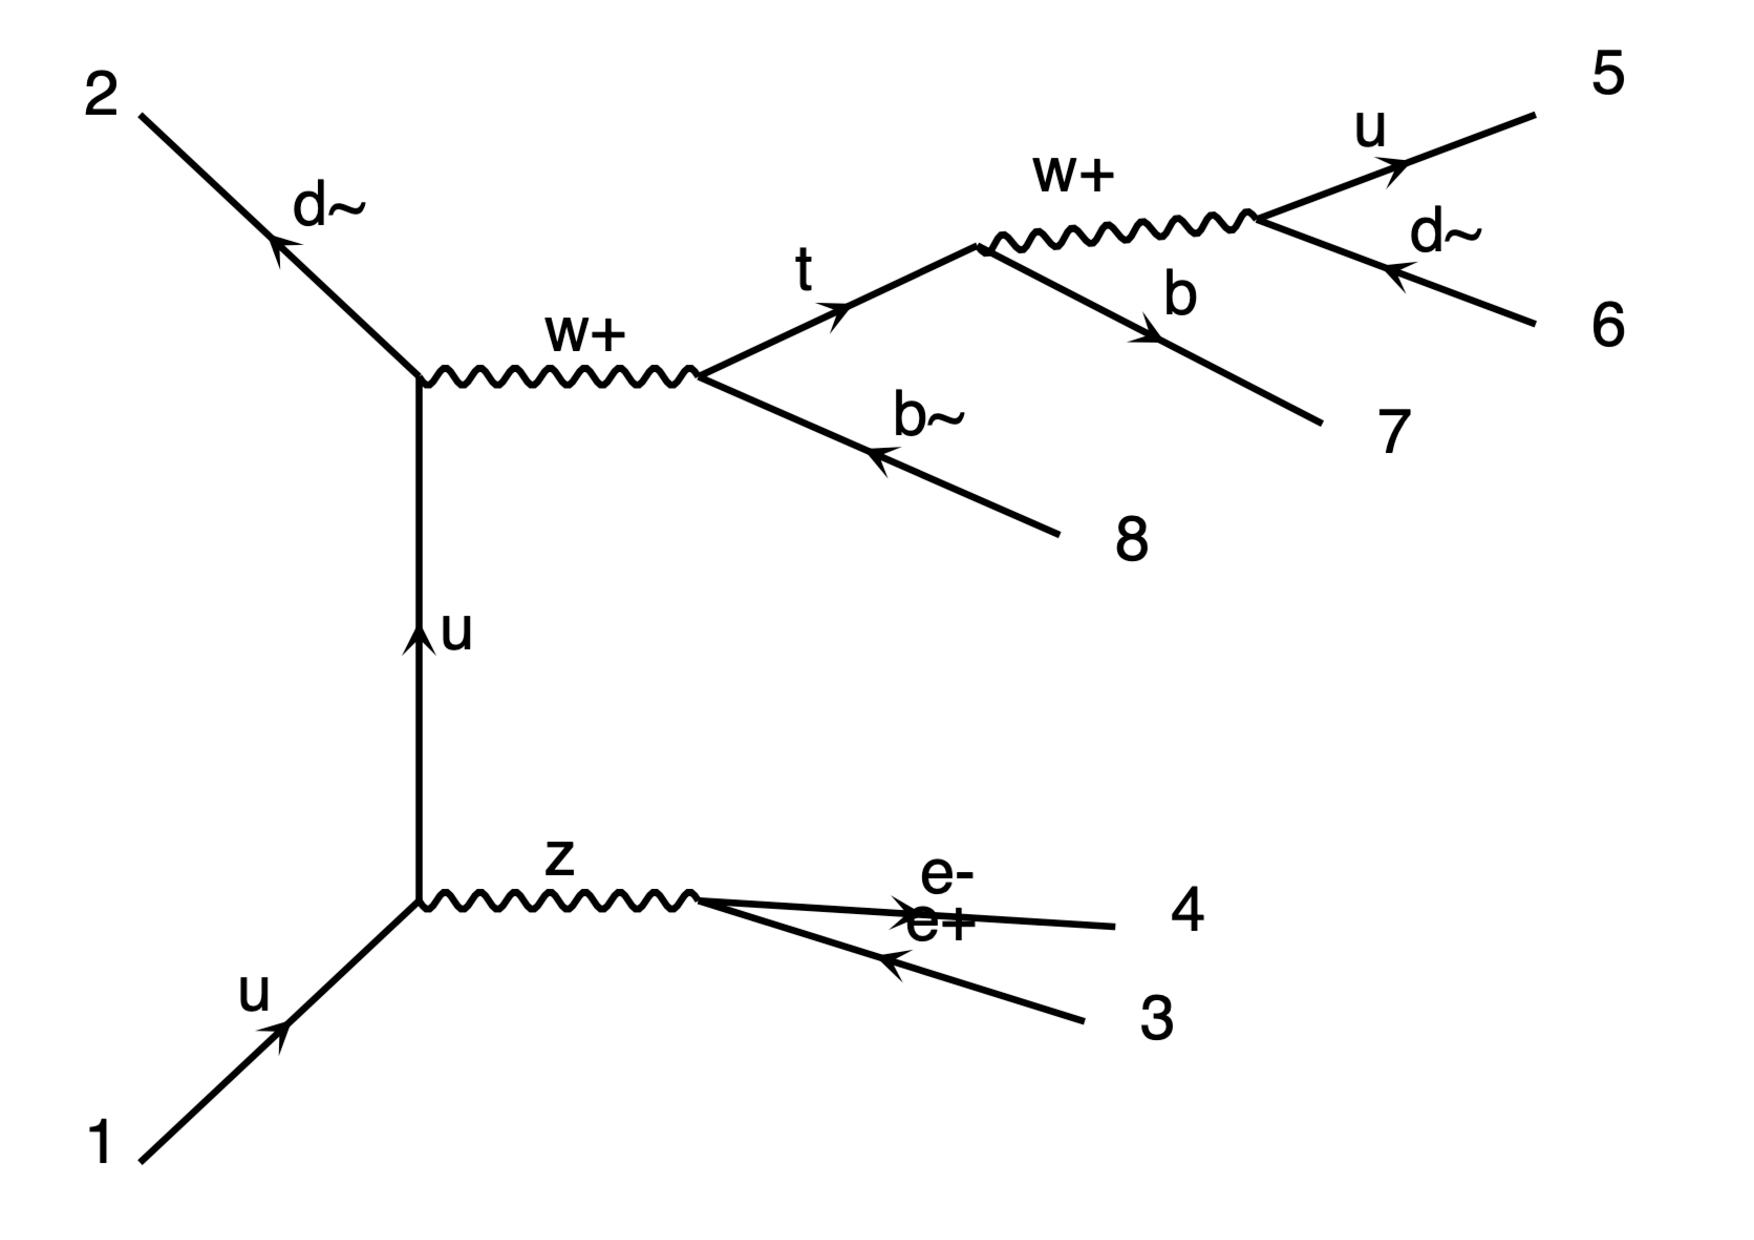
\includegraphics[width=0.5\textwidth,keepaspectratio]{figures/samples/feynEWKnonVBStZb.pdf}
\caption{
The example of the tZb diagram, which included in non-VBS diagrams.
}
\label{fig:feynmantZb}
\end{center}
\end{figure}


This contributions are reduced by applying additional cut descibed in Section~\ref{subsec:topveto}.
The production cross-section calculated by the MadGraph is shown in the table~\ref{tab:VBS_sig_samples}.
\begin{table}[!htbp]
\begin{center}
\small
\begin{tabular}{|l|l|}
\hline
Process & cross-section~(pb) \\
%\hline
%$W(l\nu)W(qq\prime)jj,b-veto$     & 1.99    \\
%$W(l\nu)W(qq\prime)jj,b-filter$   &  1.97   \\
$W(l\nu)W(qq\prime)jj$   &  3.96   \\
$W(l\nu)Z(qq\prime)jj$            &  0.25   \\
$W(\nu\nu)W(qq\prime)jj$          &  0.15   \\
$Z(ll)W(qq\prime)jj$              &  0.045  \\
$Z(\nu\nu)Z(qq\prime)jj$          &  0.032  \\
$Z(ll)Z(qq\prime)jj$              &  0.0096 \\
\hline
\end{tabular}
\caption{List of production cross sections of the signal samples.}
\label{tab:VBS_sig_samples}
\end{center}
\end{table}

The EWK VV+jj production is modeled using MadGraph5\_aMC@NLO v2.3.3~\cite{Alwall:2014hca}, plus PYTHIA8~\cite{Sjostrand:2007gs} for fragmentation.
The \textsc{NNPDF30LO} PDF set~\cite{Ball:2012cx} is used.


%\subsection{The characteristic of the VBS semi-leptonic process}
%The experimental characteristic of the VBS process is described by two vector bosons in the central region and the two jets which go forward in the opposite hemisphere.
%The kinematics of this process is illustrated in Figure~\ref{fig:VBStopology}.
%\begin{figure}[H]
%\begin{center}
%\subfigure[]{
% 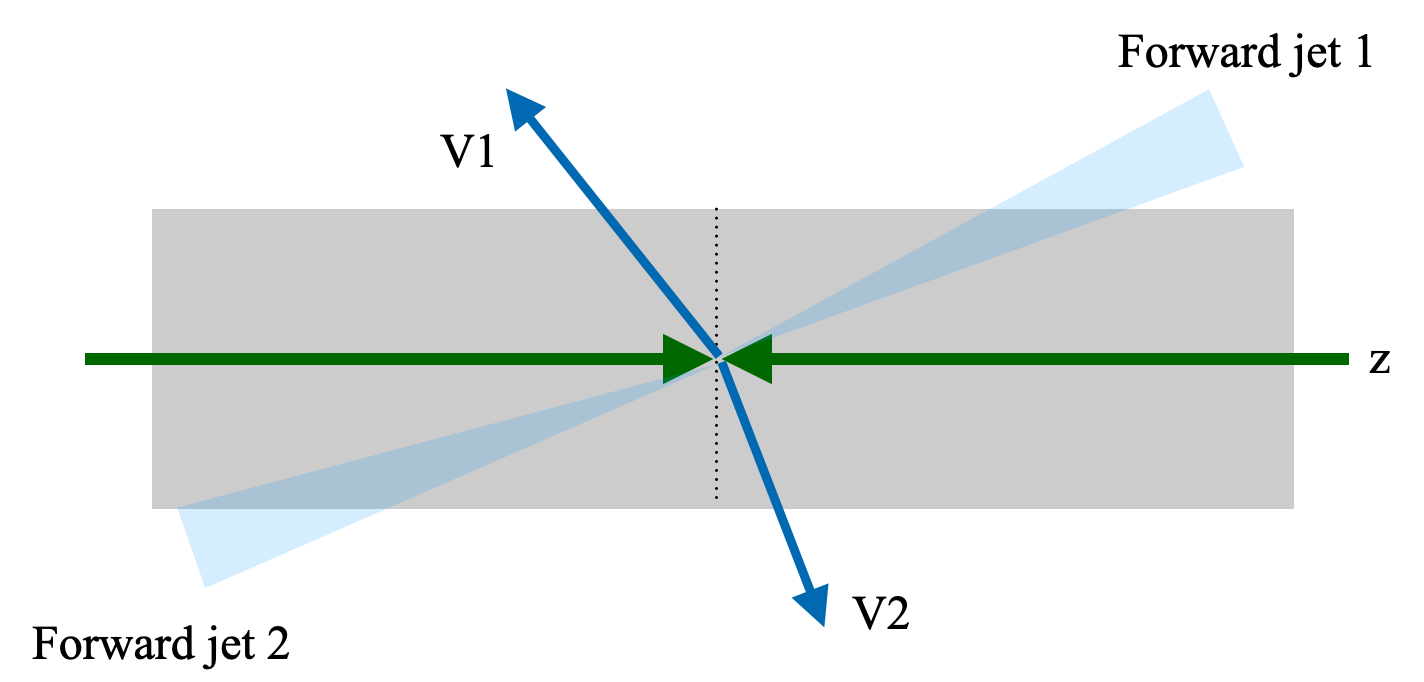
\includegraphics[width=0.75\textwidth,keepaspectratio]{figures/VBStopology}
%}
%\caption{
%The VBS topology
%}
%\label{fig:VBStopology}
%\end{center}
%\end{figure}

\section{Background process}
The Background processes in this analysis includes  $W$/$Z$ $\plus$ jets, $t\bar{t}$, single top, diboson (WW,WZ,ZZ) and multi-jets production. 

The main background for this analysis is the V($W$/$Z$)$\plus$ jets, which is the single W or Z boson in associated with jets. The final state is different with the EWVVjj signal though this is the dominant background process especially for 0-lepton and 2-lepton channel.
The V $\plus$ jets are modeled using Sherpa~2.2.1~\cite{Gleisberg:2008ta} generator. 
Matrix element is calculated for up to 2 partons at NLO, and 4 partons at LO using the Comix~\cite{Gleisberg:2008fv} and OpenLoops\cite{Cascioli:2011va}. Matrix element generators and merged with the Sherpa parton shower~\cite{Schumann:2007mg} using the ME+PS@NLO prescription~\cite{Hoeche:2012yf}.The NNPDF3.0NNLO PDF set is used in association to authors' tuning.The $W$/$Z$ + jets events are normalized to the NNLO cross sections.

The $t\bar{t}$ proceess has the same final state as EWVVjj signal process, which has two jets include b-hadron, and two W bosons decay to the leptons and hadrons. This can be the large background in 1-lepton channel, and can be reduced by requiring not to have b-tagged jets. There are minor contributions from single-top process, which is also suppressed by b-vetoing.
$t\bar{t}$ and single-top events are generated with the Powheg-Box~\cite{Alioli:2010xd} generator with the NNPDF3.0NLO PDF\cite{Ball:2014uwa} sets in the matrix element calculation.
The top quark spin correlations are preserved (for t-channel, top quarks are decayed using MadSpin~\cite{Artoisenet:2012st}). For all processes the parton shower, fragmentation, and the underlying event are simulated using \textsc{Pythia}8.230 with the A14 tune set\cite{ATL-PHYS-PUB-2014-021}. The top mass is set to $172.5\gev$. The cross sections of $t\bar{t}$ and single-top are known to NNLO in QCD including re-summation of next-to-next-to-leading logarithmic (NNLL) soft gluon terms\cite{Czakon:2011xx,Kidonakis:2011wy,Kidonakis:2010tc,Kidonakis:2010ux}.
The parameter \textsc{Hdamp} to regulate the high-\pt\ radiation in the \textsc{Powheg} is set to $1.5m_{t}$ for a good data/MC agreement at high \pt\ region\cite{ATL-PHYS-PUB-2016-020}.

The diboson processes ($WW$, $WZ$ and $ZZ$) also have the same final states with the EWVVjj signals. They are generated with Sherpa 2.2.1~\cite{Gleisberg:2008ta} generator.

All simulated events are processed with the same trigger and reconstruction algorithm as the data.The EvtGen v1.2.0 program~\cite{Lange:2001uf} is used for properties of the bottom and charm hadron decays.
Additional $pp$ collisions generated with \textsc{Pythia}~8.186\cite{Sjostrand:2008vc} are overlaid to model the effect of the pileup for all MC events.
Samples are processed through the full ATLAS detector simulation\cite{SOFT-2010-01} based on \textsc{GEANT4}\cite{Agostinelli:2002hh}.
All simulated events are processed with the same trigger and reconstruction algorithm as the data.


%\subsection{Data sets}

%\begin{table}[htb!p]
%\caption{An integrated luminosity used in this analysis. }
%\label{tab:intLumi}
%\begin{center}
%\begin{tabular}{|l|l|}
%\hline
%Year & $\mathcal{L}$ [fb$^{-1}$] \\
%\hline\hline
%2015 & 3.21 \\
%\hline
%2016 & 32.88 \\
%\hline
%2017 & 44.31 \\
%\hline
%2018 & 59.94 (21) for $\ell\nu qq$/$\ell\ell qq$ ($\nu\nu qq$) channel \\
     %& (will be updated to 58.45 with the latest lumi-tag) \\
%2018 & 58.45 \\
%\hline\hline
%total & $139.0 \pm 2.4$ \\
%\hline
%\end{tabular}
%\end{center}
%\caption{An integrated luminosity used in this analysis. }
%\end{table}

\section{aQGC signal process}



